\section{Gestaltungslösung}
\label{sec:Gestaltungslösung}

\subsection{Einleitung}
\label{sec:Gestaltungslösung_Einleitung}

Da die Grundbausteine für die Entwicklung einer optimalen Gestaltungslösung
durch die Benutzer und Aufgabenmodellierung sowie die Aufführung der Content
Elemente nun gegeben sind, geht es jetzt darum eine konkrete Lösung für das
Nutzungsproblem zu finden.
In einem Brainstorming über den groben Aufbau des Systems haben wir mehrere
Probleme identifiziert, auf die in diesem Teil der Dokumentation eingegangen
werden soll. Darunter zählen z.B. eine Standortbestimmung der Benutzer
innerhalb des Gebäudes um einen konkreten Raumvorschlag liefern zu können,
oder auch die Verifizierung der Anwesenheit von Gegenständen oder Personen
innerhalb von Räumen. Da es je nach Umfeld sein kann, dass es Räume gibt die
nicht von jeder Personengruppe genutzt werden kann oder darf, muss die
Zugangsberechtigung für Räume geklärt werden, so das gewährleistet wird das
nicht jeder Zugang zu allen Räumen hat. Außerdem muss geprüft werden wie viele
Personen sich in einem Raum gerade aufhalten um Aufschluss über die Auslastung
der Räume zu bekommen. Diese Informationen sind außerdem wichtig um
festzustellen ob ein Raum gerade belegt ist oder nicht. In diesem Teil der
Dokumentation befassen wir uns mit der Erarbeitung und kritischen Diskussion
von möglichen Technologien für einzelne Unterprobleme, die Zusammenstellung der
Komponenten des Systems und ihre Abhängigkeiten und Kommunikationsweg
untereinander.

\subsection{Kommunikation des Systems}
\label{sec:Kommunikation_des_Systems}

\subsubsection{Deskriptives Kommunikationsmodell}
\label{sec:Deskriptives_Kommunikationsmodell}

Da im aktuellen Kontext kein technisches System existiert haben wir anhand der
\ref{[Deskriptiven Aufgabenmodellierung](Textverweis)} ein Modell entwickelt,
dass die Kommunikation im aktuellen Kontext darstellen soll.

\begin{figure}[h]
	\centering
	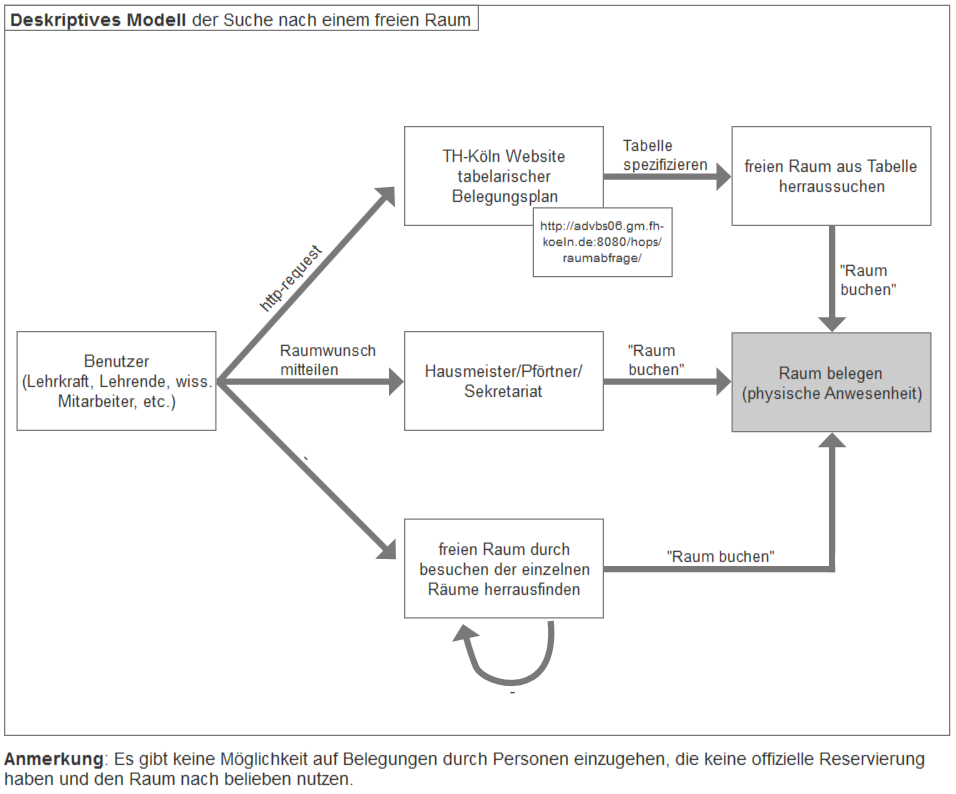
\includegraphics[scale=0.5]{deskriptiv_kommunikation.png}
	\caption{ Deskriptives Kommunikationsmodell}
\end{figure}

\subsubsection{Präskriptives Kommunikationsmodell}
\label{sec:Präskriptives_Kommunikationsmodell}

Im zu entwickelnden System haben wir uns dazu entschlossen eine REST-Konforme
Architektur zu verwenden.
Dabei basiert unsere Kommunikation auf dem Client-Server Paradigma. Wie in 
\ref{[Bild ?](client_server.png)} dargestellt hat der Client den aktiven 
Part und stellt Anfragen an den Server.
Dabei haben wir auf die Unterscheidungen der einzelnen Aufgaben geachtet.
Ein Kommunikationsaufbau vom Server zum Client halten wir in diesem Kontext für
nicht sinnvoll, da zu viele Endgeräte der Benutzer existieren um sie gezielt
durch den Server ansprechen zu können. In unserem Kontext ist dies aber auch
nicht nötig da der Server lediglich als Verarbeitungseinheit angesehen wird und
keine Anfragen an den Client senden muss.
Um REST-Konformität zu gewährleisten wird serverseitig kein Zustand gespeichert.
Jede Anfrage des Benutzers liefert alle benötigten Informationen für den Server
mit. Dazu gehören auch die Verifikation des Benutzers durch die E-Mail Adresse.
Fragt der Client einen freien Raum an, werden die E-Mail Adresse und die
eventuell benötigten Gegenstände des Benutzers im Body des Requests an den
Server gesendet. Nach einer Verarbeitung dieser Informationen sendet der Server
einen gefundenen Raum als Response an den Client zurück. Ist der gefundene Raum
an den Benutzer ausgegeben, speichert der Server diese Information in der
Datenbank. Bei Änderungen bezüglich den Status dieses Raumes, werden die
Informationen in der Datenbank aktualisiert.
Hat der Benutzer eine Raumnummer vom Server empfangen, werden diese
Informationen im Gerätespeicher des Endgerätes zwischengespeichert. Durch das
Caching dieser Informationen sind sie noch vorhanden, sollte der Benutzer die
Anwendung aus versehen schließen. Die Anwendung hat dann die Möglichkeit diese
Informationen wiederherzustellen. Um diese auf Aktualität zu prüfen sollte ein
Zeitstempel gespeichert werden anhand dem verglichen werden kann ob die Anfrage
noch aktuell ist. Damit sparen wir uns einen zusätzlichen Request zum Server um
die Aktualität zu prüfen. Die verbleibende Gültigkeitsdauer einer Information
muss dabei sowohl auf Serverseite als auch beim Client gleich sein.
Für die Adressierung der Ressourcen benutzen wir einfache Bezeichner die sich
je nach Inhalt des Bodys oder eines zusätzlichen Query String unterscheiden
lassen. Für den Hauptteil der Benutzer sind die Ressourcennamen jedoch
unsichtbar, da über eine Applikation keine sichtbare URI angesteuert wird.
Lediglich der Administrator mit einem User Interface über einen Webbrowser hat
in unserem System die Möglichkeit Einsicht in die Ressourcenbenennung zu nehmen.
Anhand der identifizierten Aufgaben aus der \ref{[Benutzungsmodellierung](Textverweis)}
haben wir eine Ressourcenadressierung vorgenommen. Die identifizierten
Ressourcen sind nicht endgültig und können sich im Entwicklungsprozess der
Gestaltungslösung oder der Implementation des vertikalen Prototyps noch ändern.
Die Auflistung der Ressourcen und ihre Adressierungen befinden sich im \ref{[Anhang](tabelle_Ressourcen.md)}.

\begin{figure}[h]
	\centering
	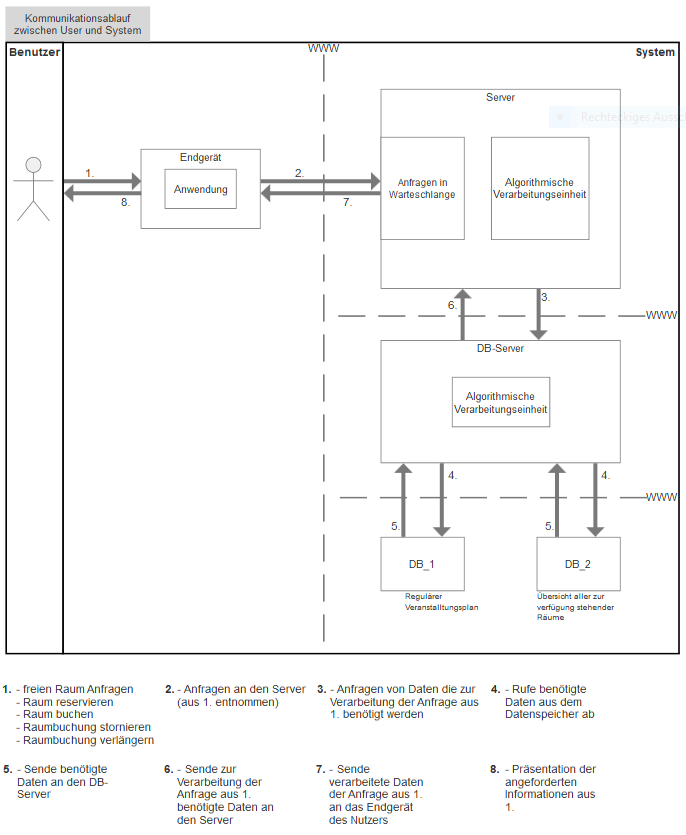
\includegraphics[scale=1.0]{praeskriptiv_kommunikation_v1.png}
	\caption{Präskriptives Kommunikationsmodell}
\end{figure}


\subsection{Architektur des Systems}
\label{sec:Architektur_des_Systems}

\subsubsection{Einleitung}
\label{sec:Architektur_des_Systems_Einleitung}
Um die Kommunikation und die Architektur der Komponenten des Systems deutlich
darzustellen, haben wir Schaubilder erstellt die es ermöglichen einen Eindruck
über unseren Aufbau des Systems zu erhalten.

\subsubsection{Deskriptives Architekturmodell}
\label{sec:Deskriptives_Architekturmodell}

Da es aktuell kein technisches System gibt auf dem wir uns in unserem Projekt
beziehen können, lässt sich auch kein deskriptives Architekturmodell ermitteln.

\subsubsection{Präskriptives Architekturmodell}
\label{sec:Präskriptives_Architekturmodell}

Um ein präskriptives Architekturmodell aufzustellen, haben wir zuerst
Komponenten identifiziert die in unserem System relevant sind.

\paragraph{Webserver}
\label{sec:Webserver}

Als Server dient uns ein über [Node.js](https://nodejs.org/en/) aufgesetzter
Webserver mit dem [Express Framework](http://expressjs.com/de/) der mittels
HTTP-Requests mit den anderen Systemkomponenten kommunizieren kann.
Da Node.js von Haus aus asynchrone Kommunikation anbietet, ist es uns möglich
mehrere Anfragen gleichzeitig auszuwerten. Der Webserver dient als zentrale
Verarbeitungseinheit für das System und behandelt alle eingehenden Anfragen der
Benutzer. Die Kommunikation funktioniert sowohl von Richtung Client als auch in
Richtung Datenbankserver über einfache HTTP-Requests die im besten Fall über
ein geschlossenes Netzwerk innerhalb der Lehreinrichtung arbeiten. Damit
besteht die Voraussetzung das der Benutzer sich im selben Netzwerk wie das
System befinden muss, \bspw über eine aktive WLAN-Verbindung. Damit würde eine
zusätzliche Authentifizierung der Benutzer erfolgen, da für gewöhnlich nur
Personen Zugang zu einer WLAN-Verbindung haben, die dort auch Mitglied oder
angestellt sind. Da aber wahrscheinlich nicht alle Lehreinrichtungen eine
WLAN-Verbindung stellen können, sollte der Zugang zum System theoretisch auch
über eine Mobilfunkverbindung mit dem Internet möglich sein.
Als Grundvoraussetzung um das System nutzen zu können, ist aber trotzdem eine
aktive Internetverbindung an die sich der Webserver anknüpfen kann. In unserem
Projekt gehen wir davon aus das die Lehreinrichtung sowohl einen verfügbaren
Internetanschluss als auch eine WLAN Verfügbarkeit überall im Gebäude
gewährleisten kann.

\paragraph{Datenbankserver}
\label{sec:Datenbankserver}

Der Datenbankserver des Systems dient als Verbindungselement zwischen Webserver
und Datenbank. Dabei liest der Datenbankserver die benötigten Informationen des
Webservers aus der Datenbank aus und leitet sie weiter. Außerdem ist er für das
abspeichern von neuen oder aktualisierten Informationen zuständig die ihm der
Webserver übermittelt.
Wir haben festgestellt das logische Unterscheidungen bei den Datensätzen
getroffen werden können. Wir haben eine logische Trennung der regulären und der
dynamischen Raumbelegung getroffen um eine eventuell bereits bestehende
Datenbank mit regulären Veranstaltungsdaten in das System eingliedern zu
können. Es bietet sich an diese auch in logisch getrennten Datenbanken
einzuordnen um eine Wartung dieser zu vereinfachen. Auf der einen Datenbank
sind nur Informationen vorhanden die bereits im Systemumfeld vorliegen,
wie \zB der reguläre Veranstaltungsplan der regelmäßig wiederkehrenden
Veranstaltungen speichert. Die andere Datenbank enthält die von uns dynamisch
erzeugten Informationen über die aktuelle Belegung der Räume durch die Benutzer
des Systems. Durch die Trennung dieser Datensätze kann je nach Bedarf der Inhalt
der Datenbanken verändert werden, ohne den Ablauf der anderen Datenbank zu
beeinflussen.
Als Datenbank haben wir uns für [Redis](https://redis.io/) entschieden, die
eine einfache Schlüssel-Werte-Datenstruktur besitzt. Da keine komplexen
Datenstrukturen benötigt werden ist diese Datenbank ideal für uns geeignet.
Ein Vorteil von Redis sind die schnellen Zugriffszeiten die bei \ca 100.000
Schreibvorgängen/s und \ca 80.000 Lesevorgängen/s liegen können was die
Bearbeitung von mehreren Anfragen vereinfacht.

\paragraph{Client}
\label{sec:Client}

Die 3. Komponente auf Clientseite ist eine Anwendung auf dem Endgerät des
Benutzers. In unserem Projekt haben wir uns auf eine Applikation, basierend auf
dem Android Betriebssystem fokussiert. Eine Umsetzung auf einem anderen
Betriebssystem, wie z.B. iOS ist aber auch denkbar, wird in diesem Projekt aber
nicht behandelt.
Laut einer Studie der [Bitkom research](https://www.bitkom.org/Presse/Anhaenge-an-PIs/2017/02-Februar/Bitkom-Pressekonferenz-Smartphone-Markt-Konjunktur-und-Trends-22-02-2017-Praesentation.pdf) 
benutzen 78\% der befragten Personen ab 14 Jahren im Januar 2017 ein Smartphone.
Mit einer Nutzerzahl von 54 Millionen Menschen in Deutschland (Tendenz steigend)
bietet es sich an das Smartphone oder Tablet in den Prozess einzubeziehen.
Zusätzlich ergibt sich der Vorteil das eine Standortunabhängige Nutzung des
Systems ermöglicht wird. So müssen nicht auf z.B. Terminals oder Anzeigetafeln
an festen Positionen im Gebäude, Informationen über Räume bezogen werden. 
Diese Anwendung stellt die Kommunikations-  und Interaktionsschnittstelle mit
den Funktionen des Systems da. Der einfache Benutzer des Systems kann durch die
Installation dieser Anwendung auf seinem Android basierten Endgerät wie \zB
Smartphone oder Tablet die Funktionalitäten des Systems nutzen. Die Anwendung
kommuniziert dabei über HTTP-Request mit dem Server des Systems und sendet
Informationen die zur Berechnung einer Raumauswahl benötigt werden.
Dabei sollte der Anwendung bekannt sein, unter welcher Adresse sich der
Webserver befindet. Um das dynamisch und auf verschiedene Lehreinrichtungen
einfach anpassen zu können, sollte unter anderem diese Adresse bei der ersten
Konfiguration in der Anwendung gespeichert werden. Da sich der Benutzer sowieso
durch z.B. Eingabe einer E-Mail-Adresse identifizieren muss, kann durch ein
zusätzliches Eingabefeld auch die Webadresse des Servers vom Benutzer erfragt
werden.

\begin{figure}
	\centering
	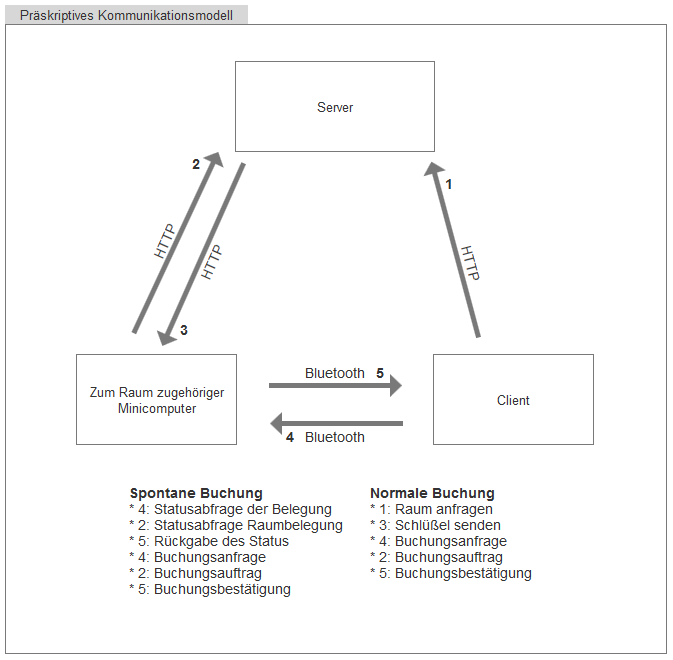
\includegraphics[scale=0.5]{praeskriptiv_architektur_v1.png}
	\caption{Präskriptives Architekturmodell}
\end{figure}

\subsection{Fazit - Architektur des Systems}
\label{Fazit_Architektur_des_Systems}

Die von uns erarbeiteten Komponenten des Systems bilden einen guten Start in
die Entwicklung. Dabei sind durch den Einsatz von Technologiebasierten Lösungen
aber noch Erweiterungen oder Änderungen zu erwarten.
Dabei ist das Systeme in einer 3-Schichten Architektur aufgebaut.
Wie in \ref{3 Schichten Architektur} gezeigt nehmen wir eine strikte Trennung
zwischen Anwendungslogik und Ressourcenmanagement vor. Das bringt uns den
Vorteil das bei Änderungen der Datenhaltung, die Anwendungslogik nicht
angepasst werden muss. Als Beispiel sei zu nennen das die Lehreinrichtung ihre
eigene Datenhaltung in das System integrieren möchte.

\begin{figure}
	\centering
	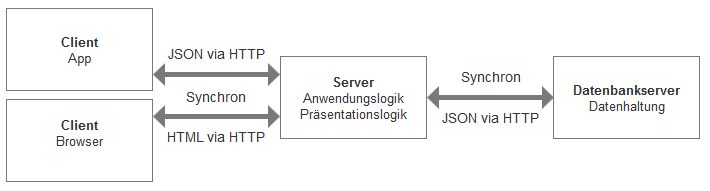
\includegraphics[scale=0.5]{3_schichten_architektur.png}
	\caption{3 Schichten Architektur}
\end{figure}

\subsection{Datenstruktur und relevante Informationen}
\label{sec:Datenstruktur_und_relevante_Informationen}

\subsubsection{Einleitung}
\label{sec:Datenstruktur_und_relevante_Informationen_Einleitung}

Um im System Informationen verarbeiten zu können, müssen diese erst einmal
definiert werden. Im Folgenden möchten wir kurz auflisten, welche Informationen
im System eine Rolle spielen und warum. Dabei unterscheiden wir zwischen
Benutzerinformationen, Rauminformationen, Filtermöglichkeiten, Belegungspläne
und sonstigen relevanten Eigenschaften.

\subsubsection{Benutzerinformationen}
\label{sec:Benutzerinformationen}

Eine Verifizierung eines Benutzers des Systems ist notwendig, da gewährleistet
werden muss, dass nur Angestellte und Mitglieder der Lehreinrichtung Zugang zu
den System- \bzw Rauminformationen erhalten. Deswegen sollte beim Systemzugriff
geprüft werden ob der Benutzer eine Zugangsberechtigung für das System besitzt.
Eine einfache Möglichkeit das zu lösen, wäre eine Authentifizierung über eine
Lehreinrichtungskennung, \zB eine spezielle E-Mail-Adresse.
Diese E-Mail-Adresse muss bei der Erstinstallation angegeben werden, und wird
bei jeder Interaktion mit dem System übertragen um den Benutzer zu
verifizieren. Der Server besitzt einen Datensatz mit berechtigten
E-Mail-Adressen, und kann so überprüfen ob die Anfrage des Benutzers bearbeitet
werden darf. Aus der E-Mail-Adresse lassen sich dann auch, \zB über das Format
der Adresse oder anhand einer weiteren Liste im System, die
Zugangsberechtigungen für bestimmte Räume prüfen. Falls die Lehreinrichtung
nicht möchte das ein bestimmter Raum von jeder Benutzergruppe genutzt werden
kann, lässt sich so eine Berechtigungsabfrage durchführen, ohne dass der
Benutzer zusätzliche Interaktionsschritte unternehmen muss. Außerdem muss der
Standort des Benutzers festgelegt werden damit er durch das System bei der
Raumauswahl berücksichtigt werden kann. Zu den infrage kommenden Technologien
dazu, kommen wir in einem \ref{[späteren Abschnitt](Textverweis)}.

\subsubsection{Rauminformationen}
\label{sec:Rauminformation}

Um einen Raum im System eindeutig identifizieren zu können, muss die Raumnummer
als Ausgangspunkt hinterlegt werden. Zusätzlich muss sämtliches, für das System
relevante, Equipment aufgelistet werden, damit im späteren Verlauf eine Suche
nach einem bestimmten Raum ermöglicht werden kann. Dieses Equipment kann je
nach Raum oder Raum Typ unterschiedlich ausfallen und hängt in der Regel von
seinem gedachten Verwendungszweck ab. Räume die für Präsentationszwecke gedacht
sind, besitzen in der Regel ein Präsentationsmedium wie etwa Beamer, Fernseher,
OHP oder Whiteboard. Zusätzlich werden, wie in fast jedem Raum,
Sitzmöglichkeiten benötigt. Die Größe, und damit die Anzahl der Sitzplätze sind
ebenfalls relevant, da nur so auf einen Raum für eine bestimmte Anzahl an
Personen hingearbeitet werden kann. Die dynamischen Rauminhalte, und mit
welchen Technologien diese aktualisiert werden können, werden im Abschnitt
[Flexible Räume](Textverweis) behandelt. Diese Rauminhalte sind je nach
Lehreinrichtung und vorhandenem Equipment variabel und müssen sich an dem
spezifischen Kontext ausrichten. Eine weitere relevante Information ist der
Standort des Raums um einen kurzen Weg zwischen Benutzer und gesuchten Raum zu
berechnen. Dieser lässt sich im Idealfall aus der Raumnummer ableiten, indem
diese so aufgebaut ist das das Gebäude, Stockwerk und der Gang daraus
ersichtlich wird. Auch diese Informationen sind variabel und müssen auf das
jeweilige Umfeld angepasst werden. Alternativ lassen sich diese Informationen
auch einzeln im System abspeichern.

\subsubsection{Filtermöglichkeiten}
\label{sec:Filtermöglichkeiten}

Damit der Benutzer nach einem Raum suchen kann, muss das System ihm die
Möglichkeit bieten auf Wünsche und Möglichkeiten einzugehen. Dazu sollte der
Benutzer die Möglichkeit haben durch spezielle Filter seinen Raumwunsch zu
konkretisieren. Diese Filter betreffen \zB den Rauminhalt der benötigt wird
damit der Benutzer seine Arbeit verrichten kann. Der Benutzer kann durch
auswählen seinen Raumwunsch eingrenzen und dem System mitteilen der diese
Wünsche in seiner Raumauswahl berücksichtigt. Der Benutzer sollte aber auch 
grundlegende Informationen angeben können, wie \zB den barrierefreien Zugang
zu Räumen. Da kann der Benutzer \zB angeben das er einen Fahrstuhl benötigt um
die Etagen im Gebäude wechseln zu können.

\subsubsection{Belegungspläne}
\label{sec:Belegungspläne}

Da in einer Lehreinrichtung oft Veranstaltungen existieren die im wöchentlichen
Muster wiederholt werden, existiert dazu meist ein Belegungsplan. Dieser gibt
an in welchem Raum in welcher Zeitspanne eine Veranstaltung, also eine Belegung
des Raumes, stattfindet. Diese Liste mit Informationen, sofern vorhanden, ist
für die Ausgabe von freien Räumen an den Benutzer eine wichtige Grundlage.
Mit ihr können viele Räume schon vorab ausgeschlossen werden, bevor sie in die
Berechnung mit einfließen. Zusätzlich muss eine Liste existieren die Auskunft
über die dynamische Belegung von Räumen Aufschluss gibt. In dieser Liste
sollten alle aktuellen Belegungen von Räumen verzeichnet sein, damit das System
bei seinen Berechnungen unterstützt wird. Die Liste sollte mit Informationen
gefüllt sein die Aufschlüsse über den belegten Raum, die Anzahl der Personen in
diesem Raum, Start- und Endzeitpunkt der Belegung sowie die
Benutzeridentifizierung des Benutzers, der den Raum gebucht hat, gibt.

\subsubsection{Sonstige Eigenschaften}
\label{sec:Sonstige_Eigenschaften}

Grundlegende Informationen wie alle zur Verfügung stehenden Räume innerhalb der
Lehreinrichtung, die Anzahl der Gebäude, Stockwerke und Gänge, Positionen von
Ein-/Ausgängen, Treppenhäuser, Notausgänge, Fahrstühle und eventuell weitere
Informationen die vom Umfeld abhängen, sind ebenfalls eine wichtige Grundlage
für das System. Mit diesen Informationen und denen der Räume und Benutzer,
können im System später Raumvorschläge z.B. für Benutzer die einen
barrierefreien Zugang benötigen erstellt werden.

\subsubsection{Fazit - Datenstruktur und relevante Informationen}
\label{sec:Fazit_Datenstruktur_und_relevante_Informationen}

Die benötigten Informationen im System sollten innerhalb eines persistenten
Datenspeichers, \bspw einem Datenbankserver hinterlegt sein. Als Datenformat
zum senden, empfangen und auswerten von Informationen, haben wir uns für das
praktische \citep{[JSON]()} entschieden. Durch die weite Verbreitung ist es ideal auf
verschiedenen Plattformen anwendbar. Die Auflistung an benötigten
Informationen und die grobe Datenstruktur befindet sich als ausführliche
Beschreibung im \ref{[Anhang](tabelle_datenstruktur.md)}.


\subsection{Standortbestimmung des Benutzers}
\label{sec:Standortbestimmung_des_Benutzers}

\subsubsection{Einleitung}
\label{sec:Standortbestimmung_des_Benutzers_Einleitung}

Damit durch unser System ein Raum ermittelt werden kann, der sowohl den
Erfordernissen des Benutzers entspricht, als auch einen möglichst kurzen
Laufweg für den Benutzer gewährleistet, muss der Standort des Benutzers
innerhalb des Gebäudes bestimmt werden.
Als Methoden zur Feststellung des Standortes haben wir verschiedene
Möglichkeiten betrachtet.

\subsubsection{Standortbestimmung durch Benutzereingaben}
\label{sec:Standortbestimmung_durch_Benutzereingaben}

Die Standortbestimmung über Benutzereingaben würde dabei so funktionieren, dass
der Benutzer einen Bezugspunkt innerhalb eines Gebäudes, z.B. eine Raumnummer
oder die Kennzeichnung eines Treppenhauses, angibt. Wir haben uns allerdings
gegen diese Methode entschieden da sie eine zusätzliche Interaktion
durch den Benutzer erfordert und das gegebenenfalls den Nutzungsfluss des
Systems stören könnte. Diese Methode kann allerdings als Fallback verwendet
werden, wenn die Standortbestimmung durch andere Methoden oder Technologien
scheitert.

\begin{itemize}
	\item Vorteile:
	\begin{itemize}
		\item Benutzer kann selber seinen Startpunkt der Suche angeben.
	\end{itemize}
	\item Nachteile:
	\begin{itemize}
		\item Benutzereingaben können fehlerhaft sein
		\item Benutzer weiß eventuell nicht wo er sich befindet
		\item zusätzlicher Interaktionsschritt durch den Benutzer nötig
	\end{itemize}
\end{itemize}

\subsubsection{Standortbestimmung durch GPS}
\label{sec:Standortbestimmung_durch_GPS}

Durch die Verwendung von GPS (Global Positioning System) könnte ebenfalls der
Standort des Benutzers bestimmt werden. Dabei würde mittels des Endgerätes des
Benutzers die Verbindung
zum "Global Positioning System" aufgebaut und somit der Standort mit einer hohen
Genauigkeit bestimmt werden. Da die Genauigkeit allerdings schwanken kann haben
wir uns gegen die Verwendung von GPS entschieden da eine fehlerhafte oder
ungenaue Messung zu falschen Ergebnissen innerhalb des Systems führen kann.

\begin{itemize}
	\item Vorteile:
	\begin{itemize}
		\item sehr präzise
		\item sehr weit verbreitet
	\end{itemize}
	\item Nachteile:
	\begin{itemize}
		\item innerhalb von Gebäuden können Signalstörungen auftreten
	\end{itemize}
\end{itemize}

\subsubsection{Standortbestimmung durch Bluetooth-Beacons}
\label{sec:Standortbestimmung_durch_Bluetooth-Beacons}

Bluetooth-Beacons sind das Indoor-Äquivalent zum klassischen GPS und
ermöglichen innerhalb von Gebäuden eine exakte Standortbestimmung auf bis zu
1 Meter \citep{insoft}.
Dazu kann eine Entfernungsbestimmung vom Endgerät des Benutzers zum Beacon
durch auslesen von Signaldaten aufgestellt werden, womit ein grober Standort
bestimmt werden kann. Durch die Bluetooth Low Energy Technik (BLE) die seit
Version 4.0 im Bluetooth Industriestandard spezifiziert wurde, sind diese
Beacons äußerst stromsparend und können dabei im Batteriebetrieb je nach
eingestelltem Sendeintervall 2-8 Jahre \citep{insoft}
senden. Durch die Möglichkeit diese an das Stromnetz anzuschließen, lässt sich
die Betriebsdauer beliebig erhöhen.
Auf dem Markt sind bereits spezielle Beacons vorhanden die für das Bestimmen
von Standorten wie \zB Messegeländen oder Flughafenterminals konzipiert worden
sind. Estimote, Inc. \citep{estimote)} 
bietet eine spezielle Lösung zu Standortbestimmung innerhalb von Gebäuden an.
Dabei lässt sich mit Hilfe eines Tools eine Karte eines Gebäudes erstellen,
auf der durch geschicktes platzieren von speziellen Estimote Beacons \citep{estimote} 
der Standort des Benutzers auf einer Karte \citep{estimote}
angezeigt werden kann. Allerdings ist diese Funktion nur exklusiv bei Estimote, Inc. \citep{estimote}
verfügbar, weswegen sie im Rahmen unseres Projektes nicht anwendbar ist.
Allerdings lässt sich ein Standort auch ohne interaktive Karte bestimmen, da
dafür nur normale Beacons benötigt werden. Die Open Source Projekt Android Beacon Library \citep{http://altbeacon.github.io/android-beacon-library/index.html}
von Radius Networks \citep{https://www.radiusnetworks.com/} biete eine
Anbindung an viele verschiedene Beacon Modelle und Marken die dem AltBeacon standard\citep{http://altbeacon.org/}
entsprechen. Über \zB eine Android Applikation lassen sich verschiedene
Informationen von einem Beacon empfangen und auslesen.

\begin{itemize}
	\item Vorteile:
	\begin{itemize}
		\item günstig
		\item einfach zu handhaben
		\item bekannte, altbewährte Technologie (Bluetooth)
		\item Langlebigkeit kann beliebig erhöht werden
	\end{itemize}
	\item Nachteile:
	\begin{itemize}
		\item Bluetooth und Wifi-Signale teilen sich eine Frequenz (2,4 GHz), kann zu Störungen führen
		\item Signaldämpfung durch Wasser und Metall im Sendebereich ist sehr hoch
	\end{itemize}
\end{itemize}

\subsubsection{Fazit - Standortbestimmung des Benutzers}
\label{sec:Fazit_Standortbestimmung}

Nach unserer Recherche, wäre das Verwenden von Beacons zur Standortbestimmung
ideal für unser Projekt geeignet. Durch die günstigen Anschaffungskosten und
die Langlebigkeit der einzelnen Beacons lassen sie sich auch in großen Massen
innerhalb eines Gebäudes anbringen. Dass die BLE Beacons sowieso schon für die
Standortbestimmung eingesetzt werden, unterstützt unsere Ansicht.
Nach unseren Erkenntnissen wäre das Anbringen eines Beacons an jedem Raum
\bzw in einem bestimmten, festgelegten Abstand von Vorteil, da dadurch eine
Beacon-Raum Zuweisung erreicht werden kann. Anhand dieser Informationen, die im
System hinterlegt sind, kann eine Standortbestimmung durch den Benutzer
erfolgen. Das Endgerät des Benutzers scannt dabei selbstständig nach Beacons in
der Nähe und speichert diese. Wenn der Benutzer einen freien Raum sucht, kann
der zuletzt gespeicherte Beacon bzw. seine ID, im Request mit übergeben werden.
Damit kann das System den Standort des Benutzers anhand des erkannten Raumes in
seiner Nähe in seine Berechnung für einen Raum mit einbeziehen. Zusätzlich kann
durch das Auslesen von Entfernungen zwischen Beacon und Benutzer eine genauere
Standortbestimmung erfolgen. Dafür muss das System die Position aller Beacons in
Abhängigkeit zu ihrem zugehörigen Raum wissen. Um diese Zuordnung einfach zu
halten, wäre es ratsam die Beacons direkt an oder über der Tür zum Raum
anzubringen. So kann erreicht werden das jede Person im Gang das Signal eines
Beacons empfangen kann. Damit Signaldämpfungen minimiert werden, sollten die
Beacons in einer Höhe angebracht werden, die über den Köpfen der Personen
liegt. Dafür würde sich der Bereich über der Tür, in \ca 2 Meter Höhe anbieten.
Um große Abstände zwischen 2 Räumen zu überbrücken, sollte in einem
festgelegten Abstand ein Beacon angebracht werden, der im System als
Pseudo-Raum zur Positionsbestimmung genutzt werden kann. Damit ein kurzer Weg
zwischen Benutzer und gewünschten Raum errechnet werden kann, müssen alle
möglichen Laufwege im System vermerkt sein. Dazu gehören auch markante Punkte
wie Treppenhäuser, Ein-/Ausgänge und Fahrstühle die ebenfalls mit einem Beacon
ausgestattet werden sollten, um die Standortbestimmung des Benutzers zu
optimieren. Für den Fall das kein Beacon durch das Endgerät des Benutzers
erkannt werden kann, sollte, sofern vorhanden, der letzte erkannte Beacon als
aktueller Standort genutzt werden. Dabei sollte der Benutzer darauf hingewiesen
werden das kein Beacon im Umkreis gefunden wurde und deshalb eine korrekte
Standortbestimmung nicht verfügbar ist. Wahlweise sollte der Benutzer die
Möglichkeit haben einen Startpunkt zu wählen, \bspw der Haupteingang des
Gebäudes. Der Einsatz von Bluetooth Beacons birgt auch einige Risiken, die wir
im \ref{[Anhang](Risiken bei der Standortbestimmung)} dokumentiert haben.
Als Ergänzung ist bei jedem Risiko angegeben wie wir mit ihm verfahren werden
sofern es eintritt. Die automatische Standortbestimmung des Benutzers ist Teil
unserer Anwendungslogik, da ohne sie die angestrebten Ziele nicht erreicht
werden können. Die suche nach Beacons erfolgt automatisch sobald die Anwendung
einmal gestartet wurde. Das Anwendungsobjekt das durch die Anwendungslogik
verarbeitet wird ist in diesem Fall eine Liste mit Beacon ID's die in der
Umgebung des Benutzers gefunden wurden. Zusätzlich wird die Liste nach dem
nächstgelegenen Beacon sortiert um bei einer Anfrage an den Server diese
Beacon ID mit zu übermitteln.

\begin{figure}
	\centering
	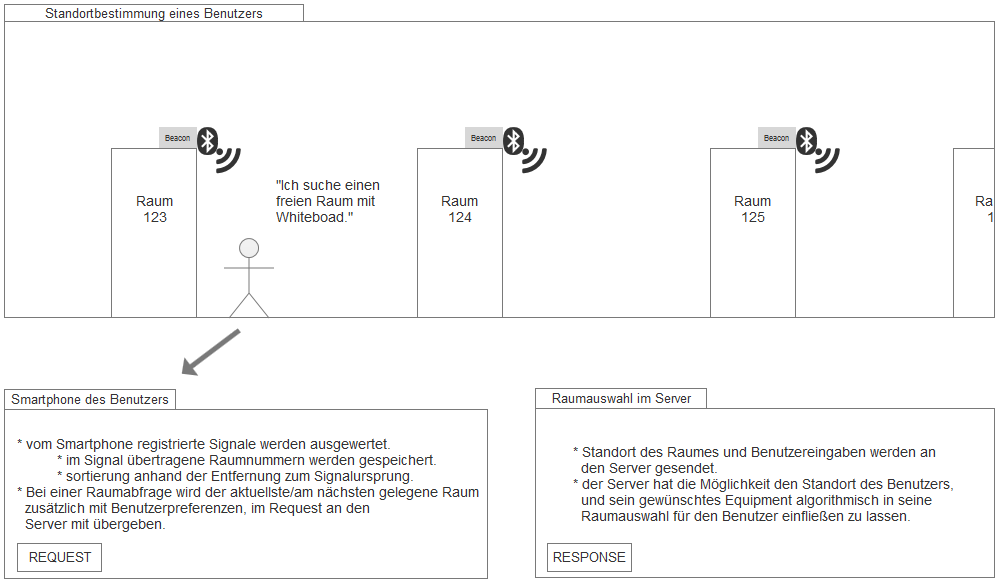
\includegraphics[scale=0.5]{standortbestimmung_beacons.png}
	\caption{Standortbestimmung durch Beacons}
\end{figure}


\subsection{Laufwegoptimierung}
\label{sec:Laufwegoptimierung}

\subsubsection{Einleitung}
\label{sec:Laufwegoptimierung_Einleitung}

Das deskriptive Aufgabenmodell der Raumsuche im Kontext der Lehreinrichtungen,
setzt das manuelle suchen von Räumen innerhalb des Gebäudes voraus. An diesem
Punkt kann viel Zeit verschwendet werden, wenn sich zusätzliche Laufwege von
Raum zu Raum ergeben, da festgestellt wird das ein gerade überprüfter Raum
schon belegt ist oder nicht das Equipment beinhaltet das vom Benutzer benötigt
wird. Das Problem hängt eng mit der Standortbestimmung des Benutzers zusammen,
da ein Laufweg immer von der aktuellen Position des Benutzers zum, vom System
berechneten, nächsten freien Raum der den Bedürfnissen und Erwartungen des
Benutzers entspricht berechnet werden muss. Im Folgenden wollen wir dieses
Problem, das unserem Alleinstellungsmerkmal entspricht, versuchen zu lösen.

\subsubsection{Verkettete Liste / Djikstra-Algorithmus}
\label{sec:Verkettete_Liste_Djikstra-Algorithmus}

Damit ein Weg berechnet werden kann, werden in unserem Fall mindestens 2 Punkte
benötigt. Zum einen der aktuelle Standort des Benutzers den wir über Bluetooth
Beacons ermitteln werden, und zum anderen der Raum \bspw die Raumnummer des
Raumes den der Benutzer benötigt. Um einen optimalen Weg berechnen zu können
muss das System Abwägungen über mehrere Räume aber auch mehrere vorhandenen
Laufwegen durchführen können.
Wir sind zu dem Entschluss gekommen das die einfachste Methode eine verkettete
Liste wäre die im System hinterlegt ist und anhand eines leicht modifizierten
Dijkstra-Algorithmus die Raumsuche übernimmt. Dabei muss für jede
Lehreinrichtung eine eigene Liste erzeugt werden die sich aus der Anzahl der
Räume, ihren Standorten und Rauminhalten sowie besonderen Merkmalen innerhalb
des Gebäudes zusammensetzt. Dabei sollte \zB der Administrator des Systems der
Lehreinrichtung, die Möglichkeit haben diese Liste jederzeit zu aktualisieren
um auf \zB Neuanschaffungen oder Umfunktionierung von Gebäuden oder Räumen
eingehen zu können.
Jeder Raum im System wird als ein Knoten innerhalb der Liste dargestellt.
Dabei sind angrenzende Knoten in der Liste gleichbedeutend mit angrenzenden
Räumen im Gebäude. So lässt sich im System ein Weg von Raum zu Raum \bzw von
Knoten zu Knoten berechnen. Wie schon erwähnt, sollten auch markante Punkte wie
Treppenhäuser oder Fahrstühle als Knoten innerhalb der Liste angegeben werden,
da sie ebenfalls als Wegstrecke zwischen zwei Punkten genutzt werden können.
Als Ergebnis enthält man eine Liste in der alle Räume und markante Punkte des
Gebäudes als Knoten modelliert wurden. Die einzelnen Knoten besitzen
verschiedene Attribute die diesen Knoten beschreiben. Jeder Knoten enthält
eine eindeutige ID die ihn innerhalb der verketteten Liste eindeutig
identifiziert. Die ID lässt sich dabei frei bestimmen und sollte
dementsprechend den Typ des Knoten kennzeichnen. \Bspw sollten Raumknoten mit
dem Präfix "room" gekennzeichnet werden, wobei ein Treppenhaus das Präfix
"stairs" beinhalten sollte. Das sorgt dafür das ein Knoten schneller und
gezielter angesprochen werden kann. Zusätzlich sollte die ID die, in der Regel
bereits bestehende, Raumnummer beinhalten. Existiert keine Raumnummer, muss der
Raum im System mit einer eindeutigen Kennung versehen werden, durch die der
Raum sich identifizieren lässt. Dabei sollte dann aber auch berücksichtigt
werden das der Benutzer eine Raumnummer oder eine ähnliche Kennzeichnung
benötigt um den Raum im Gebäude zu finden. Hierbei muss auf das gegebene Umfeld
Rücksicht genommen werden.
Ist jeder Raum im System eindeutig identifiziert und über einen Namen oder ID
in der verketteten Liste vorhanden, sollte jeder Knoten zusätzliche
Eigenschaften erhalten die für die Berechnung eines Raumes für den Benutzer
benötigt werden.
Damit ein Raumvorschlag ausgegeben werden kann, muss das System den kürzesten
Weg zwischen Benutzer und möglichen Räumen berechnen. Dabei muss das System
eine Entscheidung treffen können welcher der infrage kommenden Räume er dem
Benutzer vorschlagen sollte um einen möglichst kurzen Weg zu gewährleisten.
Um diesen Weg zu berechnen haben wir uns eine Gewichtung überlegt anhand dessen
das System den kürzesten Weg zwischen 2 Punkten berechnen kann. Jeder Knoten
besitzt die Gewichtung zu jedem seiner angrenzenden Knoten die vom Algorithmus
ausgelesen wird. Wir treffen dabei die Unterscheidung zwischen Verbindungen zu
Räumen, Treppenhäusern oder Aufzügen.
In \ref{[Schaubild 1](gewichtung_Liste_bsp.png)} ist so eine Gewichtung
schematisch zum besseren Verständnis abgebildet. Dabei ist ersichtlich das
unterschiedliche Knotentypen eine unterschiedliche maximale Anzahl an Kanten
besitzen kann. Wir haben uns auf folgende maximale Kantenzahl festgelegt:

\begin{itemize}
	\item Räume: 1-2 benachbarte Knoten/genutzte Kanten
	\item Fahrstühle/Treppenhäuser: 1-6 benachbarte Knoten/genutzte Kanten ( Norden, Süden, Westen, Osten, Oben, Unten )
	\item Ein-/Ausgänge: 1-6 benachbarte Knoten/genutzte Kanten
\end{itemize}

Um den Algorithmus sinnvoll anwenden zu können, sollte für jedes vorhandene
Gebäude mit systemrelevanten Räumen eine eigene verkettete Liste angelegt
werden. Diese Listen sollten über Einstiegs- \bzw Austrittsknoten logisch
miteinander verbunden werden. Dies ist nötig um zu gewährleisten das ein
Ausgang eines Gebäudes zu beliebig vielen Eingängen anderer Gebäude führen
kann.
Der von uns definierte Algorithmus sucht sich vom Standpunkt des Benutzers
ausgehend den Weg, der am kürzesten ist. Dabei wird immer die niedrigste Summe
der Kantengewichtungen fokussiert betrachtet. Ergibt sich auf einem anderen Weg
eine niedrigere Summe als auf dem bisherigen Weg, wird dieser Weg in den Fokus
der Raumermittlung gelegt. Der erste Raum den der Algorithmus erreicht wird als
Raumvorschlag an den Benutzer ausgegeben. 
Um nicht jeden einzelnen Weg berechnen zu müssen wird bei der Berechnung in
zwei Arten unterschieden.

\begin{enumerate}
	\item Der Benutzer und der Zielraum befinden sich in unterschiedlichen Gebäuden
	\begin{itemize}
		\item In diesem Fall wird als Zwischenpunkt der Weg zu einer Übergangsmöglichkeit gesucht.
		Es wird \zB der nächstgelegene Ausgang aus dem aktuellen Gebäude gesucht.
		Von dort aus wird die Kante zum Zielgebäude gewählt, in dem sich der Zielraum befindet.
	\end{itemize}
	\item Der Benutzer und der Zielraum befinden sich im selben Gebäude
	\begin{itemize}
		\item Trifft das zu, wird der normale Algorithmus angewandt, in dem bei allen Knoten bis
		hin zum Zielraum geprüft wird in welcher Entfernung er sich befindet.
	\end{itemize}
\end{enumerate}

Diese Unterscheidung hilft uns dabei unnötige Berechnungszeiten zu vermeiden
und effektiver Anfragen bearbeiten zu können.

Mit diesen Berechnungsmethoden für freie Räume in der Nähe des Benutzers kann
keine metergenaue Angabe gemacht werden, die Entfernung bezieht sich lediglich
auf die angegebene Gewichtung jedes Knoten. Deswegen ist eine passende
Gewichtungsangabe dringend erforderlich. Es gilt je nach Gebäude und Abstände
der Räume untereinander eine unterschiedliche Gewichtung zu legen damit eine
möglichst realistische Wegberechnung aufgestellt werden kann. Diese Gewichtung
muss je nach Anwendungsumgebung individuell festgelegt werden. Zum Beispiel
müssen Stellen berücksichtigt werden wo zwischen 2 Räumen eine größere
Entfernung vorhanden sind als normal. Die Gewichtung muss zwischen diesen
2 Knoten also erhöht werden um die erhöhte Entfernung zu simulieren.
Ein Stockwerkwechsel sollte ebenfalls mit einer speziellen Gewichtung
angegeben werden. Ein Treppenhaus bedeutet einen zusätzlichen Aufwand und je
nach Umgebung auch einen erhöhten Zeitbedarf der in Form einer erhöhten
Gewichtung berücksichtigt werden muss. Für den Spezialfall das ein Benutzer
einen barrierefreien Zugang benötigt und Räume infrage kommen die sich in
einem anderen Stockwerk befinden, wird als Zwischenziel ein Fahrstuhl oder
andere barrierefreie Möglichkeit zum Stockwerkwechsel gesucht.

\subsubsection{Fazit - Laufwegoptimierung}
\label{sec:Fazit_Laufwegoptimierung}

Die verkettete Liste mit einem Dijkstra-Algorithmus ergibt in unserem Projekt
eine sinnvolle Methode um die kürzeste Entfernung zwischen einem Start- und
mehreren Endpunkten zu bestimmen.
Das der Einsatz einer verketteten Liste in diesem Anwendungsumfeld
funktioniert, zeigt die Durchführung des Proof of Concepts den wir im \ref{[Anhang](Risiken bei der Laufwegbestimmung)}
dokumentiert haben. Durch eine Anwendungslogik wird regelmäßig automatisch
eine Liste mit aktuell freien Räumen erstellt auf die der Algorithmus
zurückgreift. Dabei verzichten wir extra auf eine vorab Berechnung aller
Routen zwischen jedem Knoten, weil damit keine dynamische Gewichtungsänderung
im laufenden Betrieb durch z.B. sperren von Gängen oder Ein-/Ausgängen
berücksichtigt werden kann.


\subsection{Flexible Räume (Verteilte Anwendungslogik)}
\label{sec:Flexible_Räume_(Verteilte_Anwendungslogik)}

\subsubsection{Einleitung}
\label{sec:Flexible_Räume_(Verteilte_Anwendungslogik)_Einleitung}

Das innerhalb von Räumen befindliche Equipment ist bis auf wenige Ausnahmen in
der Regel nicht fest installiert. So hat der Benutzer die Möglichkeit
Gegenstände von Raum zu Raum zu tragen um Räume flexibel nutzen zu können.
Im System müssen diese Verschiebungen von Equipment durch irgendeine Methode
vermerkt werden um zu gewährleisten das immer bekannt ist was sich in einem
Raum gerade an Ausrüstungen befindet. Im Folgenden sollen Möglichkeiten
diskutiert werden, die zur flexiblen Raumgestaltung eingesetzt werden können.

\subsubsection{Aktives aktualisieren von Rauminhalten}
\label{sec:Aktives_aktualisieren_von_Rauminhalten}

Zur Lösung dieses Problems muss innerhalb des Systems eine Erkennung erfolgen
die die dynamische Equipment Verschiebung erkennen und im System vermerken
kann. Die einfachste Möglichkeit wäre durch das Einbinden des Benutzers
möglich. Dabei hat der Benutzer die Aufgabe durch eine Interaktion mit dem
System Gegenstände die er aus einem Raum entfernt, aus dem Inventar des Raumes
auszutragen. Im nächsten Schritt muss er das entwendete Equipment im
gewünschten Raum zum Inventar hinzufügen. Die Umsetzung könnte innerhalb eines
einfachen Dialogs zwischen Benutzer und System erfolgen indem er den zu
entfernenden Gegenstand des Raumes auswählt und durch \zB einen Button dem
System mitteilt das dieser Gegenstand nicht länger Teil des Inventars des
Raumes ist. Im nächsten Schritt trägt der Benutzer den Gegenstand im Inventar
des Zielraums ein.
Um zu gewährleisten das der Gegenstand im gewünschten Zielraum auch wieder
eingetragen wird sollte ein durchgehender Prozess dafür sorgen das der Benutzer
nach dem Austragen eines Gegenstandes aus einem Raum als nächsten Schritt
zwingend das erneute eintragen des Gegenstandes in einem Raum vornehmen muss.
Andernfalls besteht die Gefahr das ein Gegenstand aus dem System verschwindet
und nicht mehr auffindbar ist.
Die Möglichkeit den Benutzer für diese Aufgabe einzubeziehen halten wir
allerdings nicht für optimal, da der Benutzer zusätzliche Interaktionsschritte
unternehmen muss um dieses Ziel zu erreichen. Eine automatisierte Möglichkeit
ohne den Benutzer zusätzlich zu belasten wäre zu bevorzugen.

\subsubsection{Passives aktualisieren von Rauminhalten}
\label{sec:Passives_aktualisieren_von_Rauminhalten}

Nach einer Recherche zum Thema Gegenstanderkennung \bzw Zuordnung sind wir auf
die RFID-Technologie (Radio Frequency Identification) gestoßen. Durch das
Markieren von Gegenständen und dem Anbringen eines Lesegeräts lassen sich
Gegenstände über die RFID-Technik erkennen. Dabei kommunizieren die beiden
Komponenten über elektromagnetische Wellen miteinander, die in der Regel vom
Lesegerät ausgesandt, und über kleine Antennen empfangen werden. Gleichzeitig
wird bei manchen RFID-Transpondern der benötigte Strom zum Senden von
Informationen über diese elektromagnetischen Wellen vom Lesegerät mit
übertragen. Das bringt den Vorteil das die RFID Transponder keine eigene
Stromquelle benötigen und somit passiv kommunizieren können. Beim Betreten des
Empfangsbereiches des Lesegerätes wird sowohl der benötigte Strom übertragen,
als auch Daten an das Lesegerät gesendet. Für unseren Kontext sind die passiven
RFID-Transponder ideal, da eine Vielzahl an Gegenständen mit diesen
Transpondern ausgestattet werden müssen.
Um dieses Prinzip umzusetzen muss jeder Gegenstand der relevant für das System
ist, einen Transponder und eine eindeutige ID besitzen die ihn im System
identifiziert. Es gibt verschiedene Transponder die für unterschiedliche
Einsatzzwecke geeignet sind. In unserem Fall wären flache, selbstklebende
Transponder ein Vorteil da diese schnell und einfach am entsprechenden
Gegenstand angebracht werden können. Diese Labels \citep{labels} 
kommen auch oft in der Versand und Logistikabteilung zur Anwendung um
Postsendungen oder Paletten zu kennzeichnen. Das Prinzip lässt sich auch auf
unser Projekt übertragen. Um mutwilliger oder unabsichtlicher Zerstörung diese
Labels zu verhindern, sollten diese an Positionen angebracht werden die
möglichst nicht ersichtlich sind. Die Gefahr das ein Label beschädigt und
dadurch nicht mehr erkannt wird besteht allerdings weiterhin.
Die Auswahl des entsprechenden Transponders und Lesegerätes hängt stark vom
Anwendungsgebiet und dem Umfeld ab. Unterschiedliche Frequenzbereiche können
unterschiedlich große Reichweiten gewährleisten. Diese reichen von einem
Zentimeter bis hin zu mehreren Metern. Da in unserem Fall das Lesegerät \bzw
die Antenne im Türbereich angebracht werden soll, wird eine Empfangsreichweite
von \ca einem Meter benötigt. Diese Entfernung würde man in einem
\textit{Ultra hohen Frequenzbereich} (UHF) erreichen. Diese sendet zwischen 
860 und 960 MHz \citep{[quelle](https://www.impinj.com/about-rfid/types-of-rfid-systems/)}
und erkennt selbst passive Transponder über mehrere Meter. Die UHF RFID Tags
sind dabei papierdünn, günstig und können nahezu überall angebracht werden.
Um unabsichtliches Einlesen von RFID-Transpondern im Türbereich zu vermeiden,
sollte die Antenne so ausgerichtet werden, dass sie nur von einem Türrahmen
zum gegenüberliegenden Türrahmen empfangen kann. Das anbringen des Lesegerätes \bzw
der Antenne am Türrahmen selber wäre allerdings keine gute Idee, da es möglich ist
das Personen beim Passieren der Tür die Antenne berühren oder sogar beschädigen.
Unserer Meinung nach sollte diese Antenne direkt neben dem Türrahmen wie in
\ref{[Bild ?](RFID_Lesegerät Darstellung.png)} gezeigt positioniert werden.
Um den Empfangsbereich der Antenne weiter einzugrenzen und versehentliches
einlesen zu vermeiden, wäre das Anbringen eines kleinen Reflektors um die
Antenne herum von Vorteil.

Um die erkannten Gegenstände bzw. RFID-Transponder im System zu erkennen und
Aktualisierungen zu speichern, wird als zusätzliche Komponente eine
Verarbeitungseinheit, \zB ein Raspberry Pi 3, benötigt. Das Lesegerät empfängt
dabei die erkannten Gegenstände im Empfangsbereich und sendet diese über ein
Datenkabel an den Raspberry Pi. Dieser hat in einer Liste alle
Rauminformationen inklusive aktuellem Equipment gespeichert und kann so
automatisch auf Änderungen reagieren. Wird vom Lesegerät ein Gegenstand
erkannt, wird die ID des Gegenstandes ausgelesen und an den Raspberry Pi
gesendet. Dieser gleicht die ID mit seiner vorhandenen Liste an Equipment ab. 
Ist die ID in der Liste vorhanden, also der Gegenstand ein Teil des Inventars,
trägt die Anwendung auf dem Minicomputer diesen Gegenstand aus der
Inventarliste aus. Zeitgleich wird mit der PUT-Methode ein HTTP Request an den
Server gesendet um ihn über die Aktualisierung zu informieren. Der Server liest
den Body des Requests aus in dem die Änderung (Gegenstand ausgetragen/eingetragen)
und die ID des entsprechenden Gegenstandes vermerkt sind. Der entsprechende
Gegenstand wird im Datensatz wo alle Gegenstände und ihre aktuelle Position
vermerkt sind ausgetragen. Um zu vermeiden das ein Gegenstand nach dem
Austragen im System nicht mehr vorhanden ist, wird die ID des Gegenstandes mit
dem Zeitpunkt des Austragens in eine spezielle Liste geschrieben. Auf dieser
bleibt er solange vorhanden, bis er in einem anderen Raum erkannt wird.
Somit ist gewährleistet das ein Gegenstand immer im System bekannt ist.
Das dient uns als zusätzliche Überprüfung über den Verbleib des Gegenstandes.
Der Administrator des Systems kann so regelmäßig prüfen ob Gegenstände
unterwegs abhandengekommen sind und Nachforschungen über den Verbleib anstellen.

Erkennt das Lesegerät eines Raumes einen Gegenstand der nicht Teil des
aktuellen Rauminventars ist, weiß der Minicomputer das dieser Gegenstand
den Raum gerade betreten hat. Bevor er den Gegenstand aber in seiner
Inventarliste vermerkt, fragt er den Status des Gegenstandes im System ab.
In Fehlerfällen kann es möglich sein das ein Gegenstand versehentlich Teil
eines Rauminventars geworden ist, obwohl das nicht beabsichtigt war. Wird ein
Gegenstand zu nahe an das Lesegerät eines Raumes getragen kann er
versehentlich dort in das Inventar eingetragen werden. Das kann passieren,
wenn der Gegenstand nur bis in den Empfangsbereich, aber nicht durch diesen
hindurch getragen wird. Er wird also nur einmal vom Lesegerät erkannt und dann
in das Inventar des Raumes eingetragen. Verlässt der Gegenstand den
Empfangsbereich in Richtung Ausgang, kann er vom System nicht als Gegenstand
erkannt werden der den Raum verlässt. Wird der Gegenstand dann in den
eigentlichen Raum getragen den der Benutzer beabsichtigt, würde er vom
Lesegerät erkannt und ebenfalls im Rauminventar des zweiten Raumes eingetragen.
Damit verhindert wird das ein Gegenstand im System in 2 Räumen gleichzeitig
vorhanden ist, muss eine Überprüfung erfolgen. Wenn der Gegenstand bereits Teil
eines anderen Rauminventars ist, muss er aus diesem ausgetragen und in das
Inventar des zweiten, neuen Raumes eingetragen werden. Dazu sendet der Server
dem ersten Minicomputer über einen PUT-HTTP-Request den Befehl zum Austragen
aus seinem Inventar und nach Bestätigung im Response dem 2. Minicomputer die
Erlaubnis den erkannten Gegenstand in sein Inventar einzutragen.
Den Minicomputer als Verarbeitungseinheit haben wir im \ref{[Architekturmodell](präskriptiv_architektur_v2.png)} 
und \ref{[Kommunikationsmodell](präskriptiv_kommunikation_v2.png)} ergänzt.


\subsubsection{Fazit - Flexible Räume (Verteilte Anwendungslogik)}
\label{sec:Fazit_Flexible_Räume_(Verteilte_Anwendungslogik)}

Die Überprüfung ob der Einsatz von RFID Technik für die Equipmentmarkierung in
unserem Anwendungsfeld funktioniert simulieren wir durch erstellte Datensätze.
Dabei können wir aufgrund von mangelnder Technologie aktuell nicht auf echte
RFID Transponder und Lesegeräte zurückgreifen. Um diese Technik dennoch zu
prüfen haben wir eine Simulation erstellt die überprüft ob der vorgesehene
Ablauf funktioniert. Die Dokumentation des Proof of Concepts befindet sich im
\ref{[Anhang](Risiken bei der Markierung von Gegenständen)}.
Das konkrete Anwendungsobjekt das über Anwendungslogik verarbeitet wird, ist
die Liste mit Informationen über den aktuellen Raumbestand eines Raumes.
Verändert sich die Liste durch ein- \bzw austragen von Gegenständen, wird die
Liste des Raumes auf dem Minicomputer aktualisiert. Diese aktualisierte Liste
wird dann über HTTP-Request an den Server gesendet, der diese neuen
Informationen verarbeitet und in der Datenbank in aktualisierter Form speichert.


\subsection{Verschiedene Eigenschaften der Räume}
\label{sec:Verschiedene_Eigenschaften_der-Räume}


\subsubsection{Einleitung}
\label{sec:Verschiedene_Eigenschaften_der_Räume_Einleitung}

Um im Ablauf des Systems zu gewährleisten das ein Raum auch tatsächlich frei
ist wenn der Benutzer ihn erreicht, wird eine Methode benötigt die dieses
Problem lösen kann. Im Folgenden beschäftigen wir uns mit der
Zugangsberechtigung zu einem Raum und wie der Benutzer Zugang zu diesem
bekommt. Außerdem beschäftigen wir uns mit unterschiedlichen Raumtypen. 

\subsubsection{Zugang zum Raum}
\label{sec:Zugang_zum_Raum}

Um gewährleisten zu können das ein Raum frei ist wenn der Benutzer ihn
erreicht, muss eine Zugangsberechtigung eingerichtet werden. Bei offenen
Räumen besteht die Gefahr das Personen diesen einfach belegen ohne das System
zu nutzen. Der Raum wird im System als frei angezeigt obwohl das nicht der Fall
ist. Um das Problem zu lösen wäre das generelle Abschließen aller Räume eine
Möglichkeit. Um Zugang zum Raum zu bekommen muss das System diesen gewähren
indem geprüft wird ob ein Benutzer eine aktive Reservierung für diesen Raum
besitzt. Unserer Idee nach kann das öffnen über einen vom System generierten
Code erfolgen der bei der Reservierung an das Endgerät des Benutzers gesendet
wird. Um die Tür zu öffnen muss \zB dem Minicomputer den wir in \ref{[Verweis](Textverweis)}
als neue Komponente des Systems identifiziert haben, dieser Code mitgeteilt
werden. Stimmt der Code mit dem im System hinterlegten Raum überein, kann die
Tür geöffnet werden. Um das zu realisieren muss das System sowohl dem Benutzer
als auch dem Minicomputer innerhalb des Raumes diesen Code über HTTP-Requests
mitteilen. Damit Benutzer und Minicomputer im Raum miteinander Kommunizieren
können haben wir Bluetooth und NFC als Möglichkeiten in Betracht gezogen.
Bluetooth, wie schon bei der Standortbestimmung des Benutzers verwendet, ist
eine weit verbreitete Datenübertragungstechnik die über kurze Distanz gut
funktioniert. Der im Endgerät des Benutzers gespeicherte Code wird dem
Minicomputer im Raum über kurze Distanz mitgeteilt. Der Benutzer muss sich
dabei unmittelbar vor der Tür befinden damit der Minicomputer den Code empfangen
kann. Um auszuschließen das der Code von fremden Personen abgehört und
missbraucht wird, sollte der Code im System dynamisch und zufällig generiert
werden. 

\begin{figure}
	\centering
	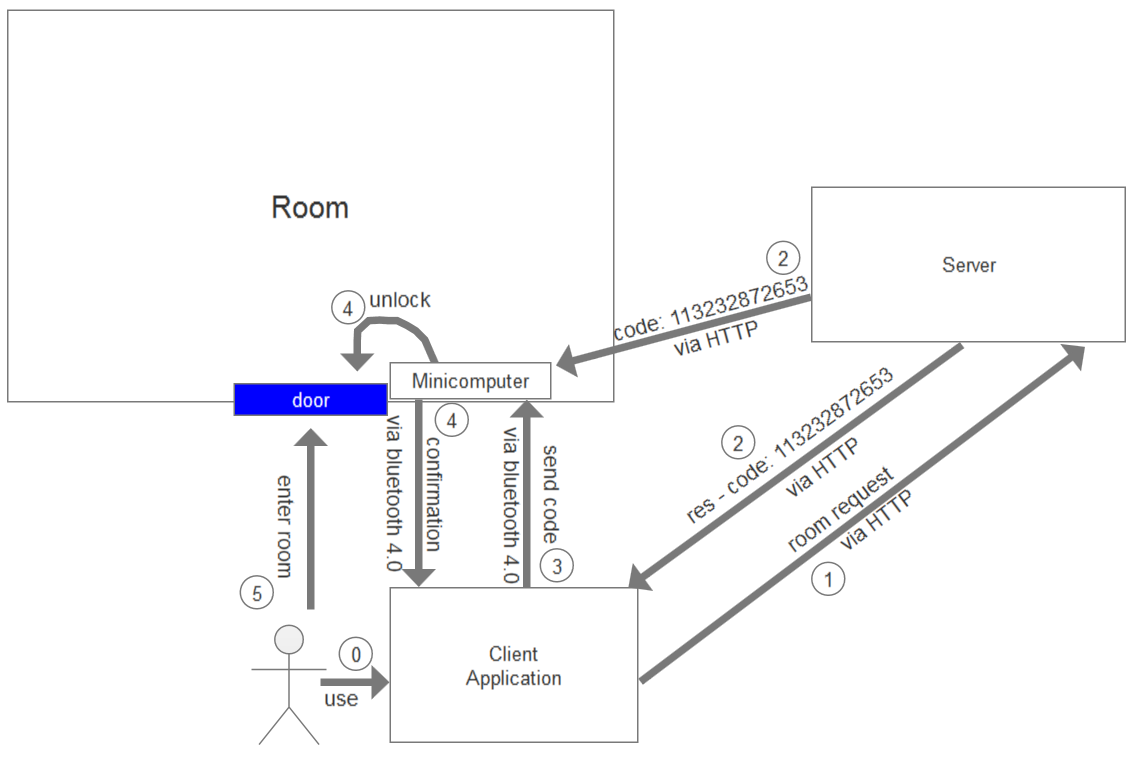
\includegraphics[scale=0.5]{zugang_zum_raum.png}
	\caption{Zugang zum Raum}
\end{figure}

Für zusätzliche Sicherheit sollte erst durch eine Bestätigung des Benutzers
dieser Code per Bluetooth an den Minicomputer übertragen werden. Damit der
Minicomputer das Bluetooth Signal empfangen kann muss das Endgerät des
Benutzers als sendender Beacon umfunktioniert werden. Durch Bluetooth 4.0 und
die Einführung der Low Energy Technik muss keine direkte Verbindung mehr
hergestellt werden was uns hier zugute kommt \cite{[Quelle](https://californiaconsultants.org/wp-content/uploads/2014/05/CNSV-1205-Decuir.pdf)}.
Eine der größeren Änderungen bei dem automatischen Entsperren der Räume ist die
Notwendigkeit das ein Computer das öffnen übernimmt. Dementsprechend muss der
Schließmechanismus so umgerüstet werden das dies automatisch erfolgen kann.
Das kann mit elektronischen Schließzylindern ermöglicht werden die in vielen
Varianten angeboten werden. In unserem Fall wäre eine drahtlose Kommunikation
zwischen Minicomputer und Schließsystem von Vorteil. Diese lässt sich ebenfalls
über Bluetooth regeln. 
NFC als Alternative zu Bluetooth funktioniert aus der Perspektive Benutzers
genauso. Allerdings muss der Benutzer sein Endgerät auf ein NFC-Sensorfeld
legen da die Kommunikation nur über wenige Zentimeter funktioniert.
Die nicht-automatisierte Alternative wäre zu akzeptieren das bei
unverschlossenen Räumen Personen den Raum einfach besetzen ohne das System zu
nutzen. Wie die Lehreinrichtung mit diesem Problem intern umgeht ist ihr selber
überlassen.

\subsubsection{Raumtyp 'Stiller Arbeitsraum'}
\label{sec:Raumtyp_Stiller_Arbeitsraum}

Da wir in unserem System einen besonderen Raum haben in denen mehrere
verschiedene Benutzer gleichzeitig und alleine arbeiten können, kann für diesen
Raumtyp die bisherige Lösung zur Raumbuchung so nicht angewandt werden.
Die besondere Eigenschaft an diesem Raumtyp bezieht sich darauf das die
Benutzer in der Regel zu unterschiedlichen Zeiten anfangen zu arbeiten und
somit eine einzige Buchungszeit kontraproduktiv wäre. Um das Problem zu lösen
sind wir zu dem Entschluss gekommen das dieser Raum ein besonderes Datenschema
benötigt. Ein Raum der zum stillen arbeiten genutzt wird, hat eine bestimmte
Slotzahl an Arbeitsplätzen zur Verfügung in die Benutzer eingetragen werden
können. Bucht ein Benutzer einen Raum zum stillen arbeiten, wird er mit dem
Zeitstempel seiner Buchung im System vermerkt. Der Raum wird wieder komplett
freigegeben wenn der letzte Benutzer den Raum nicht weiter benutzt. So kann
zusätzlich eine sinnvolle Raumbelegung erreicht werden, da dynamisch Räume zum
stillen arbeiten erzeugt und wieder entfernt werden.

\subsubsection{Fazit - Verschiedene Eigenschaften der Räume}
\label{sec:Fazit_Verschiedene_Eigenschaften_der_Räume}

Das Identifizieren und verarbeiten der Probleme "Zugang zum Raum" und dem
"Stillen Arbeitsraum" als besonderer Raumtyp haben uns dabei geholfen mehr
Lehreinrichtungen mit diesem Projekt adressieren zu können.


\subsection{Personenerkennung im Raum}
\label{sec:Personenerkennung_im_Raum}

\subsubsection{Einleitung}
\label{sec:Personenerkennung_im_Raum_Einleitung}

Zur Findung einer Methode für effektive Personenzählung haben wir ein
Brainstorming durchgeführt verschiedene Methoden betrachtet. Dazu gehören 
Methoden wie die algorithmische Personenzählung
durch Wärmebild- und Videokamera, aber auch die Erkennung durch Lichtschranken,
Druckplatten und Bewegungsmelder.
Zur Übersichtlichkeit wird in diesem Teil der Dokumentation nur kurz auf die
einzelnen Vor- und Nachteile eingegangen. Eine ausführliche Analyse der
identifizierten Technologien befindet sich im \ref{[Anhang](tabelle_Technologien.md)}.

\subsubsection{Druckplatten im Boden}
\label{sec:Druckplatten_im_Boden}

Bei der Zählung von Personen durch eine druckempfindliche Matte im
Eingangsbereich kann durch Algorithmen sowohl die Anzahl der Personen als auch
die Laufrichtung dieser durch Analyse der Drucksensoren bestimmt werden.

\begin{itemize}
	\item Vorteile:
	\begin{itemize}
		\item unauffällige Personenzählung
		\item Laufrichtung erkennbar
		\item robust
	\end{itemize}
	\item Nachteile:
	\begin{itemize}
		\item Gegenstände könnten als Personen erkannt werden
	\end{itemize}
\end{itemize}


\subsubsection{Lichtschranken und Bewegungsmelder}
\label{sec:Lichtschranken_und_Bewegungsmelder}

Lichtschranken oder Bewegungsmelder im Eingangsbereich können dafür genutzt
werden um eine Personenanzahl im Raum zu ermitteln.

\begin{itemize}
	\item Vorteile:
	\begin{itemize}
		\item keine Individuenerkennung
		\item Laufrichtung erkennbar
	\end{itemize}
	\item Nachteile:
	\begin{itemize}
		\item ungenau bei mehreren Personen gleichzeitig im Empfangsbereich
		\item keine Unterscheidung zwischen Mensch und Gegenstand
	\end{itemize}
\end{itemize}


\subsubsection{Wärmebildkameras}
\label{Wärmebildkameras}

Eine effektive Methode welche auch die persönlichen Daten der Benutzer
schützen würde wäre die Verwendung einer Wärmebildkamera mit zugehörigem
Algorithmus zur Personenzählung.

\begin{itemize}
	\item Vorteile:
	\begin{itemize}
		\item keine Individuenerkennung
		\item hohe Genauigkeit
	\end{itemize}
	\item Nachteile:
	\begin{itemize}
		\item sehr teuer in der Anschaffung
		\item Personen können durch Objekte verdeckt werden
	\end{itemize}
\end{itemize}

\subsubsection{ Video-/Bildanalyse}
\label{sec:Video_Bildanalyse}

Eine ähnliche und kostengünstigere Alternative bietet eine Analyse von
Video/- \bzw Bildmaterial mit der durch algorithmische Personenerkennung die
Anzahl der Personen ermittelt werden kann.

\begin{itemize}
	\item Vorteile:
	\begin{itemize}
		\item hohe Genauigkeit
		\item einfach in der Implementation
	\end{itemize}
	\item Nachteile:
	\begin{itemize}
		\item Personen können identifiziert werden, kein Datenschutz gewährleistet
		\item Personen können durch Objekte verdeckt werden
		\item für Videoanalyse wird ein starker Server benötigt
		\item hochauflösende Videos können nur langsam verarbeitet werden
	\end{itemize}
\end{itemize}


\subsubsection{NFC}
\label{sec:NFC}

Eine weitere Möglichkeit der Benutzererkennung innerhalb von Räumen wären der
Einsatz von NFC (Near Field Communication). 
Fast jedes neue Smartphone besitzt die Möglichkeit NFC einzusetzen. Bekannt ist
diese Methode \zB durch das kontaktlose Bezahlen mit einem Smartphone.

\begin{itemize}
	\item Vorteile:
	\begin{itemize}
		\item kontaktlose Identifikation
	\end{itemize}
	\item Nachteile:
	\begin{itemize}
		\item Reichweite stark begrenzt
		\item erfordert in der Regel Benutzerinteraktion
	\end{itemize}
\end{itemize}


\subsubsection{BLE Beacons}
\label{sec:BLE_Beacons}


Der Einsatz von Beacons wurde bereits bei der Standortbestimmung von Benutzern
angesprochen. Ebenfalls anwendbar wäre diese Methode bei der Bestimmung von
Benutzern innerhalb von Räumen.
Es wird also nach dem Standort innerhalb eines bestimmten Bereiches gesucht. 

\begin{itemize}
	\item Vorteile:
	\begin{itemize}
		\item basierend auf weit verbreitetem Protokoll
	\end{itemize}
	\item Nachteile:
	\begin{itemize}
		\item setzt Empfangsgerät beim Benutzer voraus
	\end{itemize}
\end{itemize}


\subsubsection{Fazit - Personenerkennung im Raum}
\label{sec:Fazit_Personenerkennung_im_Raum}

Nach Abwägung der Vor- und Nachteile der einzelnen Technologien sind wir zu dem
Entschluss gekommen das für dieses Projekt die Personenerkennung durch
Bildanalyse die beste Methode ist. Sie bietet eine ausreichende Genauigkeit
sofern die Kamera im Raum richtig positioniert wurde. Der Datenschutz ist
ebenfalls gewährleistet wenn die aufgenommenen Bilder ausschließlich innerhalb
des Systems verarbeitet werden. Dazu würde sich der Minicomputer innerhalb des
Raumes anbieten. Da Personenerkennung in Videos und Bildern ein aktuelles Thema
ist, kann man davon ausgehen das in Zukunft bestehende Algorithmen verbessert
oder neue Algorithmen entwickelt werden.


\subsection{Fazit}
\label{Fazit}

In unserem Projekt haben wir uns mit der Umsetzung eines Systems beschäftigt,
dass dem Benutzer Zeit sparen soll wenn er innerhalb einer Lehreinrichtung
einen Raum zum arbeiten sucht. Wir haben uns bei der Konzeption und Entwicklung
des Systems mit dem Vorgehensmodell des \citep{[Usage-Centred Design](Buch)}
beschäftigt, User Roles und Use Cases erarbeitet und diese mit Hilfe zweier
Studenten iterativ überarbeitet. Die User Interfaces für die Benutzer wurden
mit Hilfe der 5 Regeln und 6 Prinzipien der Gebrauchstauglichkeit erarbeitet
und mit zwei Studenten bewertet und verbessert. Um das Problem der zusätzlichen
Laufwege zu lösen die entstehen wenn eine Person suchend von Raum zu Raum
läuft, haben wir mit Hilfe mehrerer verketteter Listen und dem
Dijkstra-Algorithmus aus der Graphentheorie einen Algorithmus konzipiert der den
Raum mit der kürzesten Strecke zum Benutzer ermitteln kann. Um diese
Wegbestimmung zu realisieren wird der Standort des Benutzer über Bluetooth
Beacons ermittelt die in der gesamten Lehreinrichtung verteilt sind.
Dazu scannt das Endgerät des Benutzers automatisch die Umgebung nach Bluetooth
Signalen und liest die dazugehörige ID aus. Mit ihr weiß das System wo der
Benutzer sich befindet, und kann so eine realistische Berechnung aufstellen.
Um auch Gegenstände innerhalb von Räumen in der Raumauswahl zu berücksichtigen
haben wir die Möglichkeit einer Markierung von Gegenständen durch RFID-Tags in
Betracht gezogen. Dabei wird durch ein Lesegerät im Eingangsbereich eines jeden
Raumes überprüft ob ein Gegenstand den Raum verlässt oder betritt. Dadurch wird
eine dynamische Verschiebung von Equipment zwischen verschiedenen Räumen
ermöglicht, was die Raumgestaltung flexibler gestaltet. Um zu überprüfen ob
sich Personen innerhalb eines Raumes aufhalten womit der Status des Raumes
festgelegt werden kann, haben wir uns für die Bildanalyse entschieden.
Unserer Meinung nach wurden alle aufgestellten Ziele adressiert und deren
Erfüllung im System durch Einsatz verschiedener Technologien und Prinzipien
erläutert.
Bei den von uns betrachteten Technologien ergaben sich viele interessante
Möglichkeiten die aber teilweise im aktuellen Projektkontext nicht anwendbar
waren. Sollten sich die ermittelten Probleme in näherer Zukunft beheben, wären
auch Technologien wie Druckplatten im Boden als Personenerkennung eine
brauchbare Methode.
\citet{ISO9126}
